
\documentclass[review,3p,times,authoryear,12pt]{elsarticle}
\usepackage{amsmath,amsthm,amssymb}
\usepackage{algorithm}
\usepackage{graphicx,subfigure}
\usepackage{clrscode}
\usepackage{enumerate}
\usepackage{multirow,endfloat}
\graphicspath{{figure/}}
\newtheorem{proposition}{Proposition}

\begin{document}
\begin{frontmatter}
\newpage
\title{A Heuristic for the Stowage Stack Minimization Problem with K-Rehandle Constraint under the circular route}
\begin{abstract}
The container stowing planning have been investigated widely from different aspects considering different objectives.
In our previous research, we proposed the stowage stack minimization problem(SSMP)which investigated a stowage planning problem when carriers have the obligation to ship all the given containers in different ports, with the objective to utilize the fewest
number of stacks on the ship.
In this paper, we talk about SSMP with K-rehandle constraint in circular routes for container ships, abbreviated as CSSMP.
A heuristic algorithm is proposed to construct solutions.
We conduct experiments on lots of instances generated by computer according to practical operations of container shipping.
Our heuristic algorithm shows better performance comparing with the random heuristic.
\end{abstract}
\begin{keyword}
Containership stowage planning\sep circular routes\sep stack minimization \sep K-rehandles \sep constructive heuristic
\end{keyword}
\end{frontmatter}

\section{Introduction}
% to do:
%1.introduce the importance of containership transpotation.
%2.introduce the container stowage planning.
%3.introduce the circular routes and ship structure.
%4.introduce what we did and what the contributions are.
%5.introduce the contexts of next chapters.

The increasing demand for maritime transportation of containers have led to the construction of numerous mega container vessels, many of which have the capacity to carry more than 18,000 twenty-foot equivalent units (TEU) containers.

In a container ship, a stack is obtained by stacking containers vertically, several stacks in a row form a bay, and bays are placed side by side to form a container block, which is called bay-row-tier system.

In a general case, container ship serves many different ports on each voyage.
A stowage planning for container ship made at one port must take account of the influence on subsequent ports.
Therefore, the complexity of stowage planning problem increases due to its multi-ports nature.

In the linear routes discussed in \cite{wang2014stowage}, the destination port of container is larger than the origin port of containers.
Due to the characteristic of circular routes, there are different kinds of containers at each port to be loaded.
For example, some containers are loaded in the current round and discharged in the next round.
we have to design more data structure to store different container types and simulate different loading and unloading situations.
\section{Literature review}
% to read and review literatures
\cite{ambrosino2015mip} proposed a Mixed Integer Programming (MIP) heuristic aimed at determining stowage plans in circular routes for container ships so as to give support for the ship coordinator and the terminal planner.
%To the best knowledge of us, it was the first time circular routes had been considered into this kind of problem.


\section{Problem description and properties}
We put forward CSSMP in this section, it is a variant of containership stowage planning problem (CSP) in the nature.
In the circular routes, a ship starts its journey at port 1 and sequentially visits port 2, 3, ..., $P$, 1, 2, 3, ... until the ship stops.
We call it a round from port 1 to port $P$ and assume the ship stops after $R$ rounds.
In each round, $N$ containers are shipped and containers are discharged and loaded at each port.
We use $O(c)$ and $D(c)$ to denote the original and destination ports of container c in the actual description, respectively.
Accordingly, the itinerary is represented by a tuple $\{O(c), D(c)\}$.
However, we have to use $O'(c)$ and $D'(c)$ to denote the original and destination ports of container c in our algorithm since containers in the current round can be transported into the next round.

In our stowage stack minimization problem with K-Rehandle constraint in the circular routes, the whole routes of the ship is investigated; in particular, different sets of containers must be loaded for being shipped to the next ports at each port of the route.
The sequence of two handling operations has an important influence on the effectiveness of a stowing plan: first, the import containers must be unloaded from the ship, then the export containers can be loaded.

Given a ship with its structural characteristics, its route, described by a circular sequence of ports to be visited, and its current cargo, the problem consists in defining the stowage plan for a given set of containers that differ for the loading and destination port, so that all the containers are loaded on board, while the structural and operative constraints are satisfied and the number of stacks used on the vessel at the ports for loading/unloading operations is minimized.

Each ship travels on a circular route with P ports and the transport demand is randomly generated in such a way that for each origin port in the route of a ship.
For example, if P equals to 6, when planning the stowage for port 5, the ship has on board a cargo deriving from loading operations executed at ports 1, 2, 3 and 4. At port 5, after that the unloading operations are executed, the loading process regards containers bound for port 6, 1��, 2��, 3�� and 4��, where 1��, 2��, 3�� and 4�� denote the port 1, 2, 3 and 4 reached during the second round of the ship.

There are some assumptions for the convenience of our research:
\begin{itemize}
\item	All the containers have the same size, twenty-foot equivalent units (TEU) containers;
\item	Containers at each port for each loop have the same quantities and types;
\item	The vessel has a limit height considering the security and balance of the vessel;
\item	After the unloading and loading operations at each port, there are at most K rehandles exist;
\item	The voyage should stop at a certain loop after we have found the convergence.
\item	Other constraints to ensure the security of vessel are satisfied.
\end{itemize}

\clearpage

\subsection{Integer model}

\clearpage

\section{Methodology}
\label{sec:algo}
In this section, we will talk about the heuristic algorithm to solve the CSSMP as well as the performance guarantee of the algorithm.

\subsection{Heuristic algorithm for the SSMP}
\label{sec:h1}
We first give some related notations for ease of exposition.

\begin{itemize}
\item $R$ means the circle number of rounds.
\item $K$ means the number of rehandles limited in each layout in our problem.
\item $k$ means the number of real rehandles and it ranges from zero to $K$.
\item $nearport\_s$ represents the value of the nearest port of stack $s$.
\item $NumofStack\_r\_p$ is referred as the number of used stacks after the ship's departure from port $p$ in the $r-th$ round.
\end{itemize}

Here is a simple example to illustrate $nearport_s$.
Three containers are stored in stack $s$, and their destination ports are 4, 5, 6, respectively, then the value of $nearport_s$ is 4.
In particular, the value of $nearport_s$ of every empty stack $s$ is set as $2*P$.


We have constructed a heuristic algorithm which greedy rules are adapted.
There are main three procedures in our algorithm: unloading, sorting and loading.
Considering the existing of rehandles, our strategies to handle loading and unloading operations are different.
The rules become strict when it comes to meeting the conditions that there are certain rehandles constraints.
However, the main ideas are extremely similar.
The stacks on the vessel are divided into different categories according to whether rehandle will occur when the loading container is loaded into the stack.
Hereafter, we give them different priority to reduce the number of used stacks as much as possible.
The priority of them is following:
\begin{itemize}
\item Partial stacks with no rehandles occurring.
\item Partial stacks with rehandles occurring.
\item Empty stacks.
\end{itemize}
Obviously, the first choice will be removed if the problem meet the constraints with zero rehandle.

Algorithm \ref{alg:1} solves instances of CSSMP.

\begin{algorithm}[htbp]
  \caption{A heuristic algorithm for the CSSMP}
  \label{alg:1}
  \begin{codebox}
  \Procname{\proc{Heuristic(I)}}

    \li \For each round $r=1, 2, \ldots,R $
    \li \For each port $p=1, 2 , \ldots,P $
    \li \Do
                execute method $unloading\_at\_port(p)$.
    \li         Sort containers with $O(c)==p$ by the decreasing order of their destinations.
    \li         \For each container $c$ with $O(c)==p$
    \li         \Do
                   \If $k==K$
    \li            \Then
                        execute method $loading\_equalK(c)$.
    \li            \Else If $k < K$
    \li                 execute method $loading\_lessK(c)$.
                   \End
                \End
    \li          figure out the value of $NumofStack\_r\_p$.
        \End
        \End
    \li Output the results of all instances.
 \end{codebox}
 \end{algorithm}

\subsubsection{Detail description of unloading method}
\label{sec:d1}

\

\noindent A ship calls at port $p$, some containers are supposed to be discharged.
We should find out those containers to be unloaded firstly according to $D(c)==p$.
Afterwards, whether there are blocking containers are placed on the target container is judged.
We will discharge blocking containers and reset their values of original ports if there exists blocking containers.
Of course we can discharge target container directly if there are no blocking containers.
At last, we update the  height of the stack which the target container is discharged from.

\subsubsection{Detail description of loading methods}
\label{sec:d2}

\

\noindent Two different methods based on our greedy rules are adopted to choose stack for each loading container according to the relationship between $k$ and $K$ when loading containers at each port.
They are called as $loading\_lessK(c)$ and $loading\_equalK(c)$, respectively.
The detail description of the two loading methods will be introduced in this section.

We firstly talk about the simple condition when $k==K$.
In the $loading\_equalK(c)$ method, we first consider choosing a stack from partial stacks with $nearport_s \ge D(c)$ for container $c$.
If there are no such partial stacks exist, then one empty stack is necessary.
Therefore, the stack selection priority for container $c$ under this condition is:

\begin{enumerate}
\item the set of partial stacks, each container $s$ in which satisfies the constraint that $nearport_s \ge D(c)$.
\item the set of empty stacks.
\end{enumerate}


Afterwards, we talk about the complex condition when $k < K$.
In the $loading\_lessK(c)$ method, the kinds of feasible stacks increase as a result of the existence of rehandles.
Under this condition, the stack selection priority for container $c$ becomes:

\begin{enumerate}
\item the set of partial stacks, which is indexed as $S_1$, each container $s$ in $S_1$ meets the constraint that $nearport_s \ge D(c)$.
\item the set of partial stacks, which is indexed as $S_2$, each container $s$ in $S_2$ meets the constraint that $nearport_s < D(c)$.
\item the set of empty stacks, which is indexed as $S_3$.
\end{enumerate}

Both in method $loading\_equalK(c)$ and $loading\_lessK(c)$, we need to clear all sets of stacks once we have chosen a stack for each loading container at every port.
Of course, we will update the value of $k$ if there is a rehandle when loading containers.
After loading the current container into the chosen stack $s*$, the height of $s*$ and $nearport_s*$ should both be updated.

Actually, a lot of variables and methods of the specific unloading and loading strategies have been involved, we do not write all of them here for the sake of context length.

\subsection{Random algorithm for the SSMP}
\label{sec:r2}
Apart from the heuristic algorithm, we also design a random algorithm to construct solutions to get the container stowage planning.

The main three procedures in the random algorithm are also unloading, sorting and loading.
The difference between the heuristic algorithm and random algorithm is the loading method and we will talk the loading method of the random algorithm in detail.

When a ship calls at a port, the target containers are discharged and the blocking containers are reset sorted with the onshore containers.
After sorting containers, we begin to load containers one by one.
When we choose a stack for the current loading container, we judge the all stacks by sequence.
First, the stack can't be a full one.
Second, if rehandle occurs, we need to judge whether there are rehandles allowed;
if no rehandle occurs, we just choose the current stack that we are discussing.
Third, update the height of chosen stack and the number of rehandles in current layout.



\clearpage

\section{Experiments and Analysis}
For each containership, five instances have been generated; each instance differs from the others for the transport demand to satisfy.
Anyway, all instances have been generated in such a way to stress the capability of the heuristic approach to obtain feasible and effectiveness solutions in a short amount of time.

We divide our instances into three parts according to the size of limit height: Small Ship with H equals to 4 and N is selected from {100,400}; Medium Ship with H equals to 8 and N is selected from {1000}; Large Ship with H equals to 12 and N equals to 2000.

The following figures will show us the results of heuristic algorithm:

\begin{figure}[htbp]
\centering
\setlength{\abovecaptionskip}{10pt}
\resizebox{1.0\textwidth}{!}{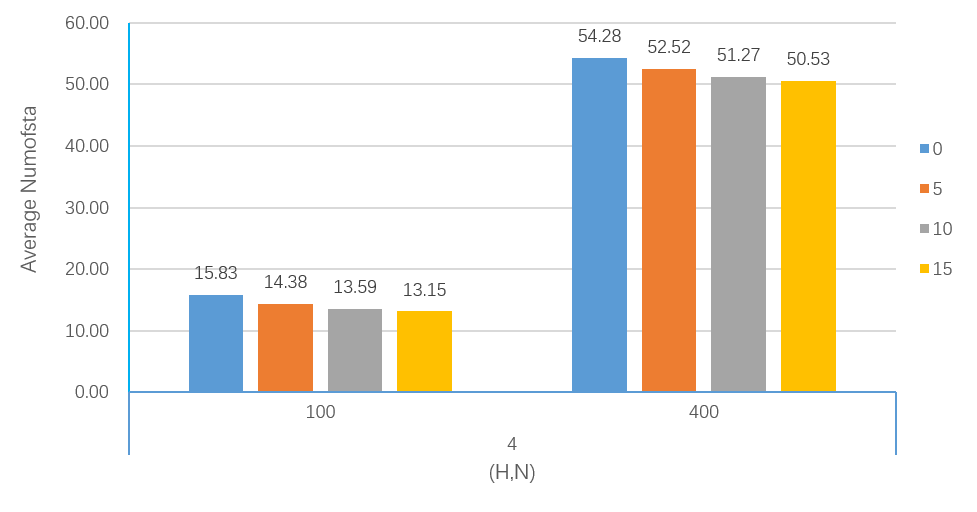
\includegraphics{figure/heu/small.png}}
\caption{Results of small size in heuristic algorithm.}
\label{fig 1:graph}
\end{figure}

\begin{figure}[htbp]
\centering
\setlength{\abovecaptionskip}{10pt}
\resizebox{1.0\textwidth}{!}{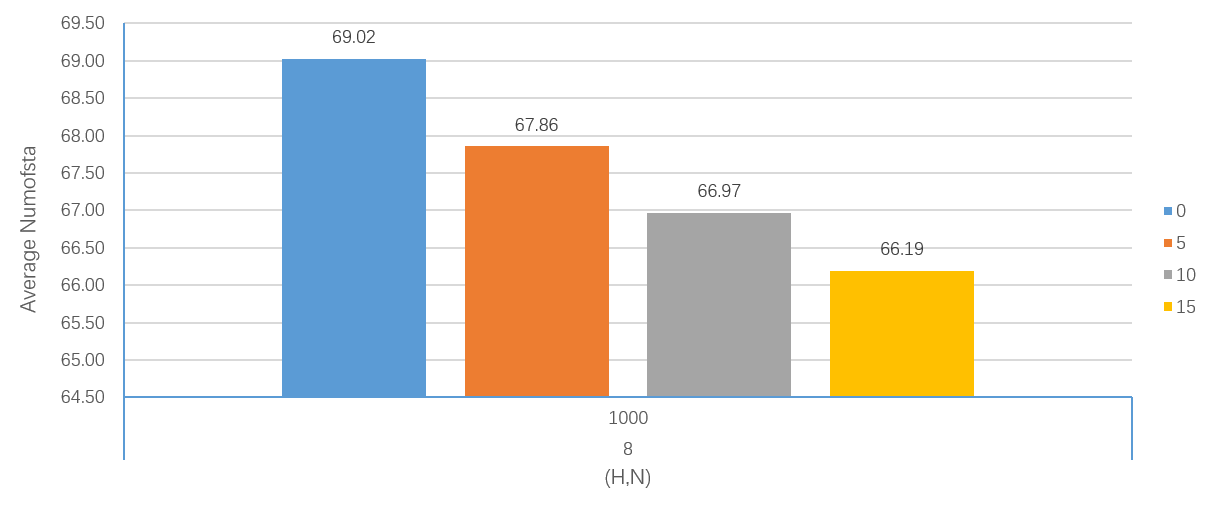
\includegraphics{figure/heu/medium.png}}
\caption{Results of medium size in heuristic algorithm.}
\label{fig 2:graph}
\end{figure}


\begin{figure}[htbp]
\centering
\setlength{\abovecaptionskip}{10pt}
\resizebox{1.0\textwidth}{!}{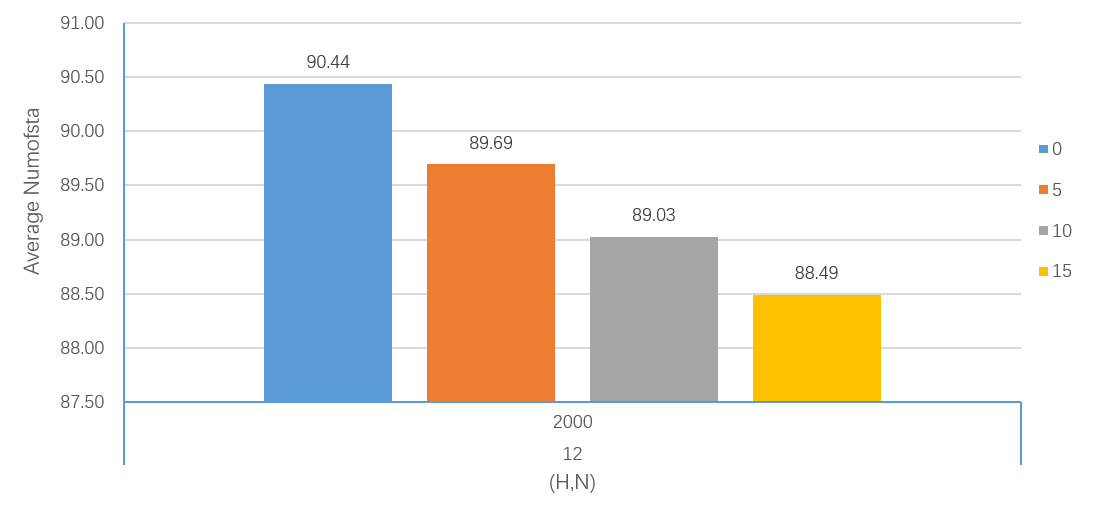
\includegraphics{figure/heu/large.png}}
\caption{Results of large size in heuristic algorithm.}
\label{fig 3:graph}
\end{figure}

\begin{figure}[htbp]
\centering
\setlength{\abovecaptionskip}{10pt}
\resizebox{1.0\textwidth}{!}{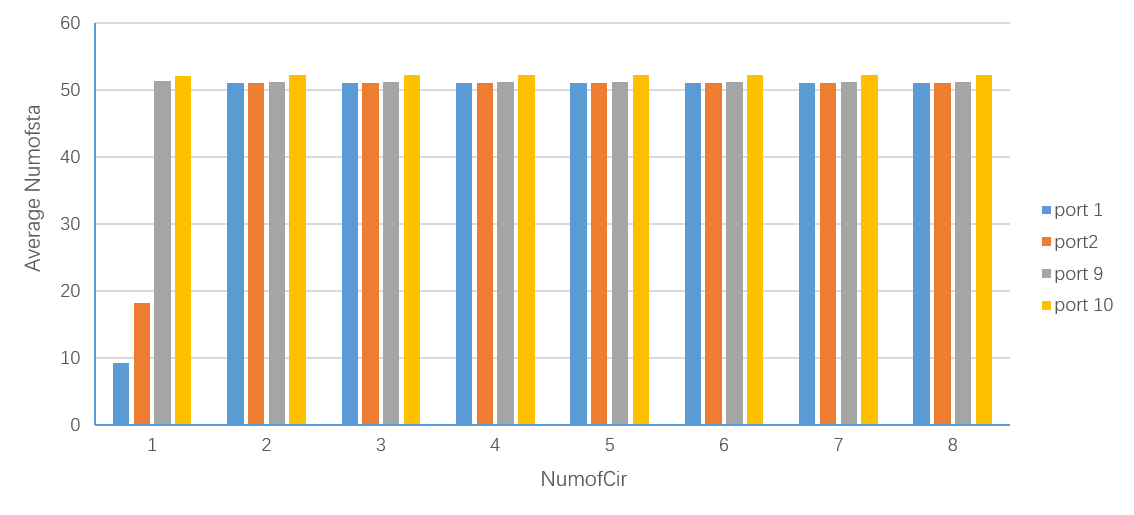
\includegraphics{figure/heu/cir-port.png}}
\caption{Relationship between loop and port with small size in heuristic algorithm.}
\label{fig 4:graph}
\end{figure}

\begin{figure}[htbp]
\centering
\setlength{\abovecaptionskip}{10pt}
\resizebox{1.0\textwidth}{!}{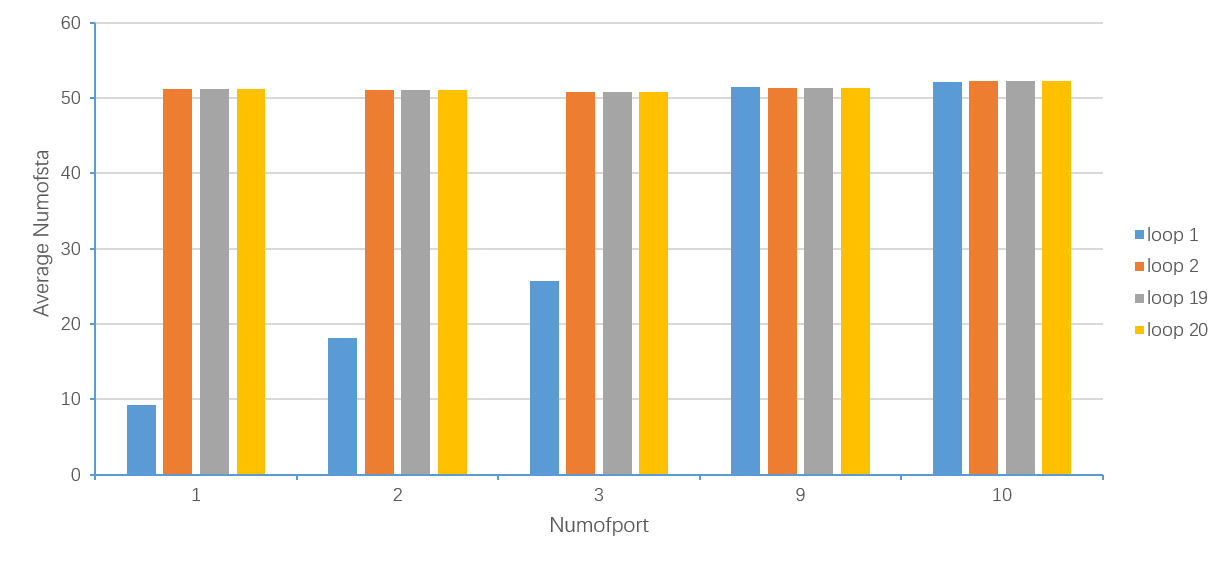
\includegraphics{figure/heu/port-cir.png}}
\caption{Relationship between port and loop with small size in heuristic algorithm.}
\label{fig 5:graph}
\end{figure}

\begin{figure}[htbp]
\centering
\setlength{\abovecaptionskip}{10pt}
\resizebox{1.0\textwidth}{!}{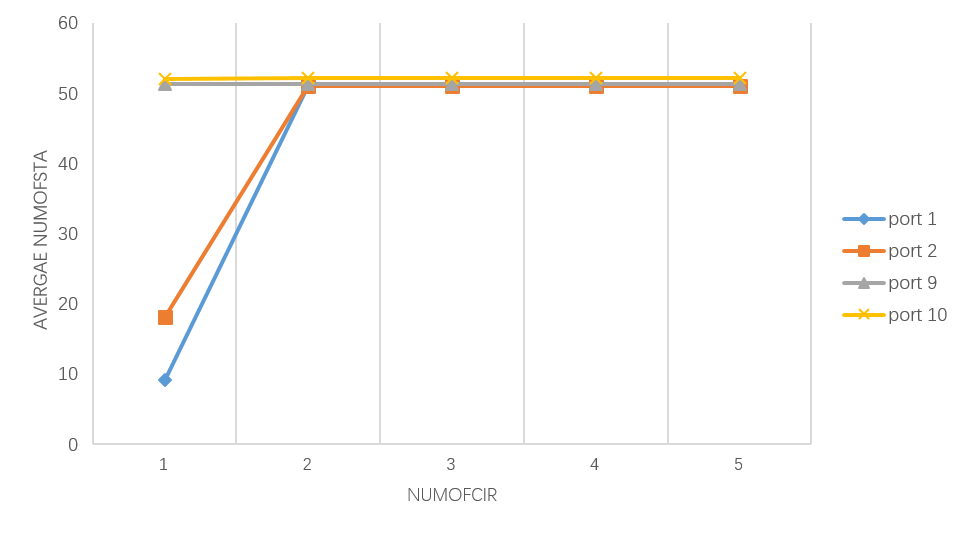
\includegraphics{figure/heu/zhexian.png}}
\caption{line chart of relationship between port and loop in heuristic algorithm}
\label{fig 6:graph}
\end{figure}


The following figures will show us the results of heuristic algorithm:
\begin{figure}[htbp]
\centering
\setlength{\abovecaptionskip}{10pt}
\resizebox{1.0\textwidth}{!}{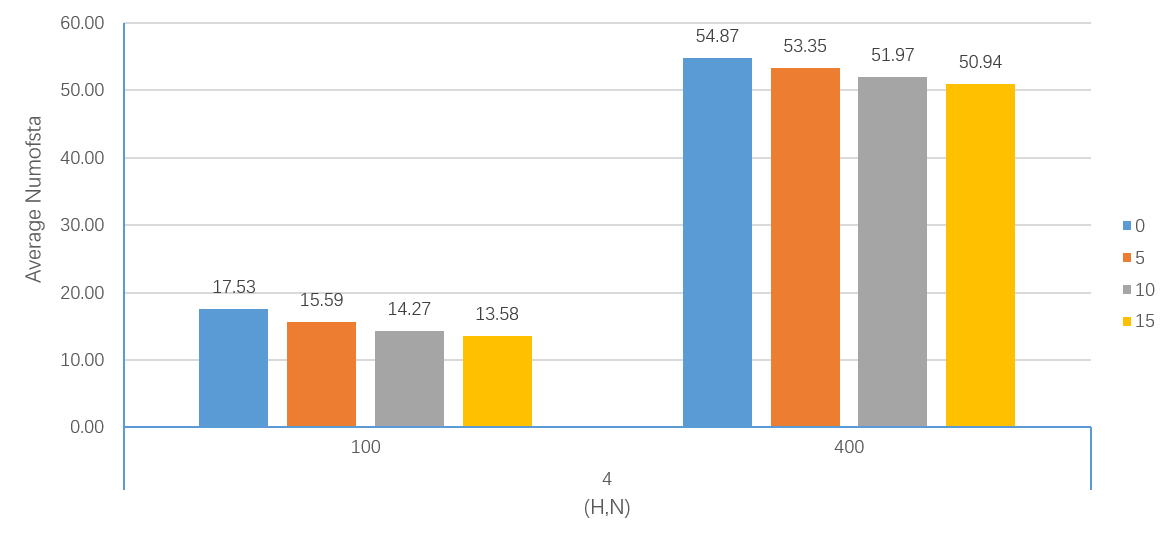
\includegraphics{figure/ran/small.png}}
\caption{Results of small size in random algorithm.}
\label{fig 7:graph}
\end{figure}

\begin{figure}[htbp]
\centering
\setlength{\abovecaptionskip}{10pt}
\resizebox{1.0\textwidth}{!}{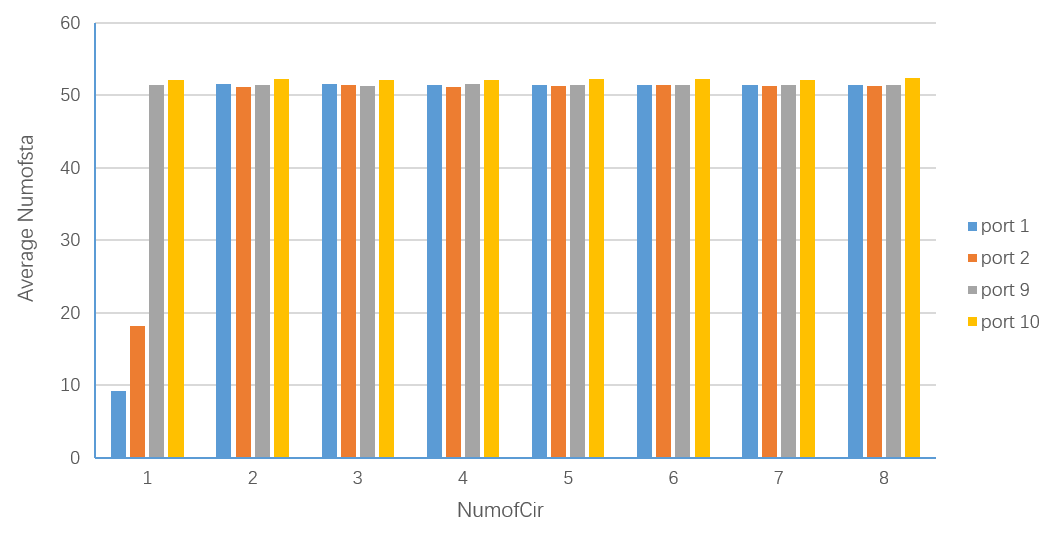
\includegraphics{figure/ran/cir-port.png}}
\caption{Relationship between loop and port with small size in random algorithm.}
\label{fig 8:graph}
\end{figure}

\begin{figure}[htbp]
\centering
\setlength{\abovecaptionskip}{10pt}
\resizebox{1.0\textwidth}{!}{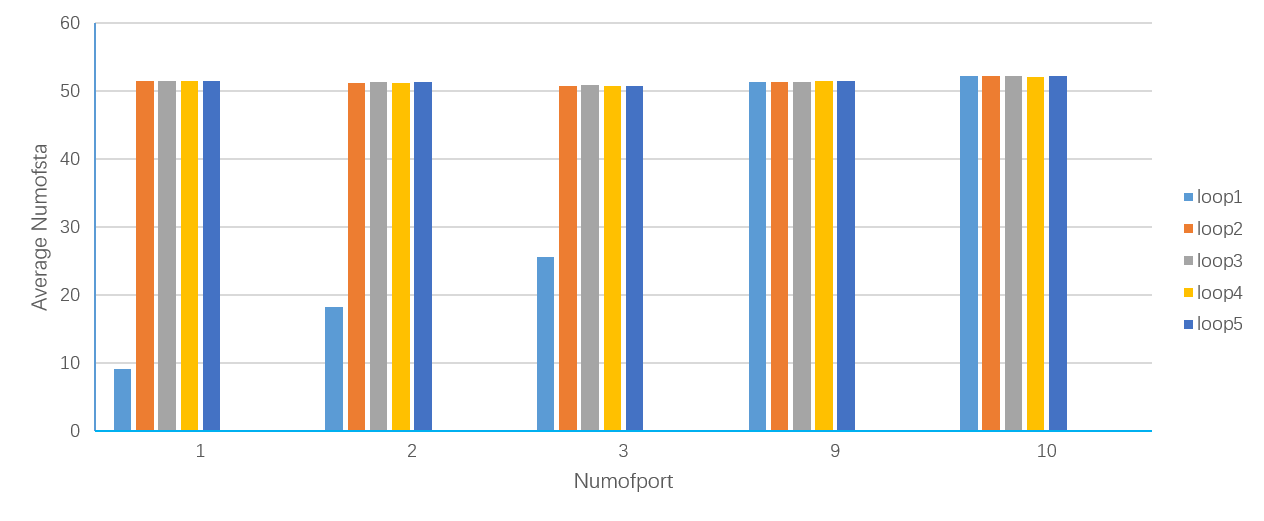
\includegraphics{figure/ran/port-cir.png}}
\caption{Relationship between port and loop with small size in random algorithm.}
\label{fig 9:graph}
\end{figure}

\begin{figure}[htbp]
\centering
\setlength{\abovecaptionskip}{10pt}
\resizebox{1.0\textwidth}{!}{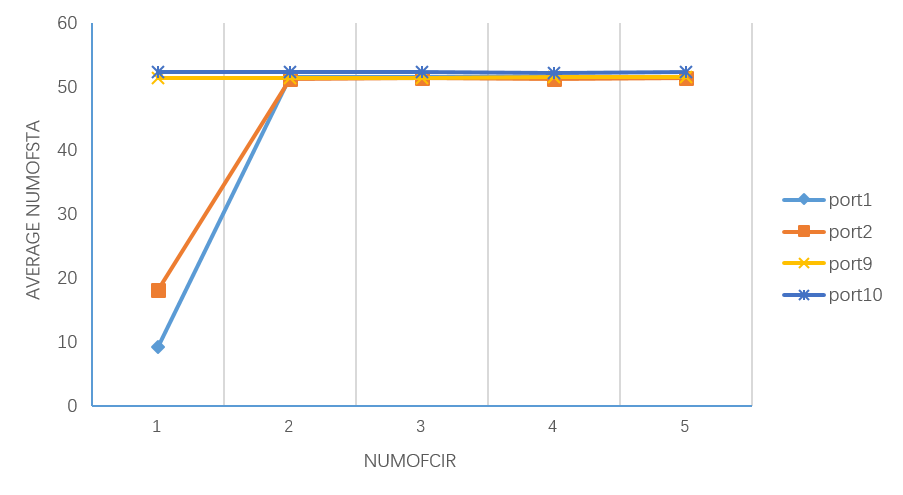
\includegraphics{figure/ran/zhexian.png}}
\caption{line chart of relationship between port and loop in random algorithm}
\label{fig 10:graph}
\end{figure}

We get the following conclusions after analysing our experiments results.
\begin{enumerate}
\item The last port and the second last port in the first loop converge faster than other ports.
      The theoretical guarantee should be proved.
\item Apart from minority of instances, the number of used stacks at every port in most instances converge to a certain value
and stop changing.
\item The distribution of the number of used stacks of multi ports in the first loop is extremely different from the second loop.
After a certain number of loops, the distribution remains unchanged.
\item For some instances, the number of used stacks in every port can converge faster if there is no rehandle.
When there are a certain number of rehandles constrainted, layouts will remain unchanged after volatility.
\item Instances with the same parameters but different seeds have a strong influence on the number of used stacks. What��s more, the influence is dynamic with the different parameters.
\end{enumerate}

We also get some propositions for our conclusions.

\begin{proposition}
The last port and the second last port in the first loop converge faster than other ports.
\end{proposition}

\begin{proof}
The last port and the second last port, no matter what the loop is, the containers at port are the
same because there are not containers from the last loop in their layouts after unloading and loading operations all the time.
However, the other ports are different since the layout in the first loop is different from the layouts in other loops.
Hence, the last port and the second last port in the first loop converge faster than other ports is proved.
\end{proof}

\begin{proposition}
The distribution of the number of used stacks of multi ports in the first loop is extremely different from the second loop.
\end{proposition}

\begin{proof}
It is not difficult to draw the second conclusion.
In the first round, there is not containers from the last round at all ports.
After the first round, the layouts of some ports contains two types of containers and the number of used stacks increases.
\end{proof}

\begin{proposition}
the number of used stacks is no greater than $\lceil\frac{2*N_p}{H}\rceil$.
\end{proposition}

\begin{proof}
Considering the characteristics in the circular route, the upper bound of our problem becomes $\lceil\frac{2*N_p}{H}\rceil$ since the number of containers at a single port can��t reach 2*N.
\end{proof}

\clearpage

\section{Conclusion}
We take the circular routes into account in this paper and we construct heuristic algorithm to work out  the stowing planning.
The experimental results show that our problem considering circular routes is of practice and its results
could be used to decision support for forwarders.

\bibliographystyle{apalike2}
\bibliography{Cir_SSMP}
\end{document}
